\section{Camera modelling} \label{sec:camera_modelling}
A central problem when working with camera-generated images and 3D models is
correctly mapping 3D points in camera (and world) frames into 2D points on the
acquired camera's image and viceversa. In particular, the capability to map
points of the world to a generalized camera model in a realistic way allows all
the algorithms, such as point cloud alignement, to work within a generalized,
global coordinate system, which remains valid also if cameras are moved around
within the scene and is camera-independent: this means that different cameras
can be used in order to maximimize the peculiarities of each. Also, virtual
renders can be done using the same model in order to correctly template-match
the chosen data.  A \emph{pinhole} camera model can be used for this task, and
provides the correct approximation for both RGB cameras and depth-capable ones.

\subsection{Pinhole model for registered RGBD cameras}\label{sec:intrinsics}
A camera, be it a digital camera or the human eye, can be modeled by
considering the path the light coming from a point will take when
captured. By approximating the camera's objective with a single point (hole),
light rays come onto projective plane (where the light sensor is), which is at a
distance $f$ (called \emph{focal length}) from the hole of the camera; light
travels with central
simmetry with respect to the position of the point in world coordinates. By
rotating the $(u,v)$ reference frame of the image so that it has the same
orientation as the image seen by the camera \footnote{Notice that the image
  coordinate system the $V$ axis is pointing downwards; this is coherent both
  with standard screen coordinate systems, which have the origin in the
  upper-left corner, and with having the camera $Y$ axis pointing downwards and
$Z$ axis pointing forward.}, the point corresponding to the camera hole
becomes the destination point for all the light paths, as seen in single-point
prospective. This transformation is called \emph{perspective projection}.

\begin{figure}[htbp]
\centering
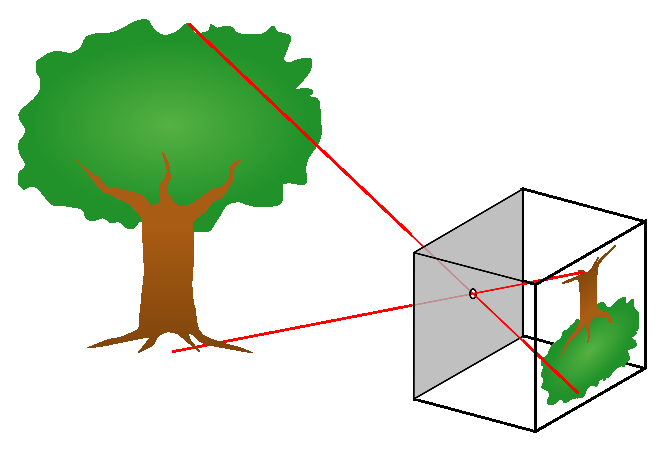
\includegraphics[width=2.5in]{./Graphics/pinhole_camera}
\caption{The pinhole camera model \label{fig:pinhole_camera}}
\end{figure}
\begin{figure}[htbp]
\centering
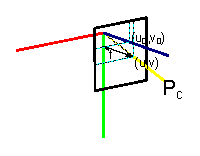
\includegraphics[width=2.5in]{./Graphics/camera_intrinsics}
\caption{Geometric projection of a general point into the camera's projective
plane. \label{fig:intrinsics}}
\end{figure}
Examining the geometric properties of this system from fig. \ref{fig:intrinsics}, we can easily extract the
transformation from a point $P_c(x_c,y_c,z_c)$ in the local coordinate system
$X_cY_cZ_c$ to the corresponding point $P_p(u,v)$ in the image's coordinate
system by applying trivial similar triangles' laws:

\[
  \begin{array}{c}
    \left\{\begin{array}{c}
    \frac{(u-u_0)}{\lambda _x f}=\frac{x_c}{z_c} \\
    \frac{(v-v_0)}{\lambda _y f}=\frac{x_c}{z_c}
  \end{array}
  \right. \\
  \Updownarrow \\
  \left\{\begin{array}{c}
      u=\left(\frac{x_c f}{z_c}\right) \lambda _x+u_0 \\
      v=\left(\frac{y_c f}{z_c}\right) \lambda _y+v_0
    \end{array}
    \right. 
  \end{array}
\]

Here, $\lambda _x$ and $\lambda _y$ are camera-dependant ratios between the
physical sensor's dimensions and its horizontal and vertical resolution, in
order to map coordinates from meters to pixels. These can be merged into $f$ to
get $f_x$ and $f_y$.

Also, as we are assuming to work with a registered RGBD image, $z$ coordinate is
directly measured from the depth sensor and is reported on a per-pixel basis
without the need of further processing.

If we use \emph{homogeneous coordinates} as described in sec.
\ref{sec:homogeneous-coordinates}
to describe both 3D and 2D points, we get

\begin{equation} \label{eqn:intrinsics}
\left(\begin{array}{c}u\\v\\z_c\end{array}\right)
  =
  \left(\begin{array}{cccc}
      f_x & 0 & u_0 \\
      0 & f_y & v_0 \\
      0 & 0   & 1 
  \end{array}\right)
\left(\begin{array}{c}x_c\\y_c\\z_c\end{array}\right)
\end{equation}

We call the matrix 
$K=
  \left(\begin{array}{cccc}
      f_x & 0 & u_0 \\
      0 & f_y & v_0 \\
      0 & 0   & 1 
\end{array}\right)$
the \emph{intrinsic} camera matrix. This matrix incorporates all the
characteristics which are proper of the used camera, and is different for each
camera -- also of the same model -- as it depends on small build details too,
such as lens geometry.

\subsection{Global camera transformation}
By using the matrix derived in section \ref{sec:intrinsics}, points from 2D
images can be brought into a reference system centered into the camera.
By considering the relative transformation between the world's frame and camera
frame, we can move those points into global coordinates to be further
manipulated from other algorithms in a camera-agnostic way.

If we consider $E$ to be the relative pose between world and camera, we have
(again, using homogeneous coordinates):

\begin{eqnarray}
  E&=&\left(
  \begin{array}{c}
  R | T \\
  0 | 1
\end{array}
\right) \\ 
\nonumber \\
\left(\begin{array}{c}x\\y\\z\\1\end{array}\right)
  &=&
  E
\left(\begin{array}{c}x_c\\y_c\\z_c\\1\end{array}\right) \label{eqn:extrinsics}
\end{eqnarray}

The matrix $E$ is called \emph{Extrinsic camera matrix}.

\subsection{3D cloud reconstruction from RGBD image}
\label{sec:cloud-reconstruction}
By inverting eqns. \ref{eqn:intrinsics} and \ref{eqn:extrinsics} we can pass from homogeneous
$(u,v,z_c)$ coordinates to homogeneous $(x,y,z)$ coordinates. In practice, this
means passing from points into a camera-generated image to a cloud of points in
the global coordinate system.

\begin{equation}
  \left(\begin{array}{c}x\\y\\z\\1\end{array}\right)
  =E^{-1}K^{-1}\left(\begin{array}{c}u\\v\\z_c\end{array}\right)
\end{equation}

\subsection{Calibration of camera parameters}
Calibration is the process of extracting the intrinsic and extrinsic
camera matrix for a camera. It is done through the analysys of a serie of RGB and depth
frames containing a single, known object with known size and features. In
particular, a big chessboard pattern has been chosen for this work.

Intrinsic camera matrix can be obtained by using the built-in
\texttt{calibrateCamera} OpenCV's feature. %TODO ref
Before calling it, the pattern's features can be found using the corresponding
facilities like \texttt{findChessboardCorners}. This function examines a serie
of $(u,v)$ points corresponding to the features as they are seen from multiple
frames and multiple pattern's poses, and tries to minimize the RMS error on a
fitness function considering the relative position between these features. Care
must be paid in order to cover the whole camera space when taking frames, thus
minimizing the total error on the intrinsic matrix computation.

In order to compute efficiently the extrinsics matrix, an original program has
been developed in order to exploit depth information too, which is not used at
all by OpenCV's builtins. First, the chessboard corners are located using the RGB
channels of the image. After this, they are sorted so that the point with the
lower $u$ and higher $v$, i.e. the one in the bottom-left corner, is point
number 0, and proceeding left to right. Each point is then mapped to its 3D
camera coodinates $(x_c,y_c,z_c)$ using equation \ref{eqn:intrinsics}. 

Points associations between camera and global coordinates are done
bidirectionally: point 0 is associated to global origin, and point N to global
coordinate $(x_n, y_n, 0)$.

As points' correspondances are univocal, we can use the ideas presented in
\cite{extrinsics-algorithm}, which introduce a closed-form algorithm for finding
the optimal transformation between the points. First, we find the two points sets' relative
translation by computing the distance vector between the points' centroids:
\begin{equation}
  T=\frac{1}{N}\sum_{i=1}^{N}(P^i-P_c^i)
\end{equation}

After this, we align the two centroids into the origin and use Singular Value
Decomposition to find the optimal rotation:
\begin{eqnarray}
  H &=& \sum_{i=1}^{N} (P^i - C)(P_c^i - C_c)' \\
  \left[U,S,V\right] &=& SVD(H) \\
  R &=& VU'
\end{eqnarray}

Finally, the error can be computed and tested to be low enough. If the result is
good, the theoretical and captured chessboard are correctly aligned as shown in
fig. \ref{fig:extr_alignment}.

Both intrinsic and extrinsic matrices are saved to a camera model file by the
calibration programs.

\begin{figure}[htbp] 
\centering
\begin{tabular}{c|c}
  \adjustbox{valign=m}{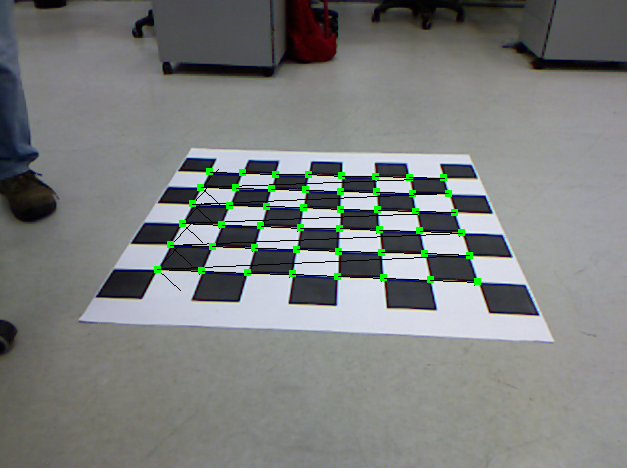
\includegraphics[width=2.5in]{./Results/Chessboard_points_cut}} &
  \adjustbox{valign=m}{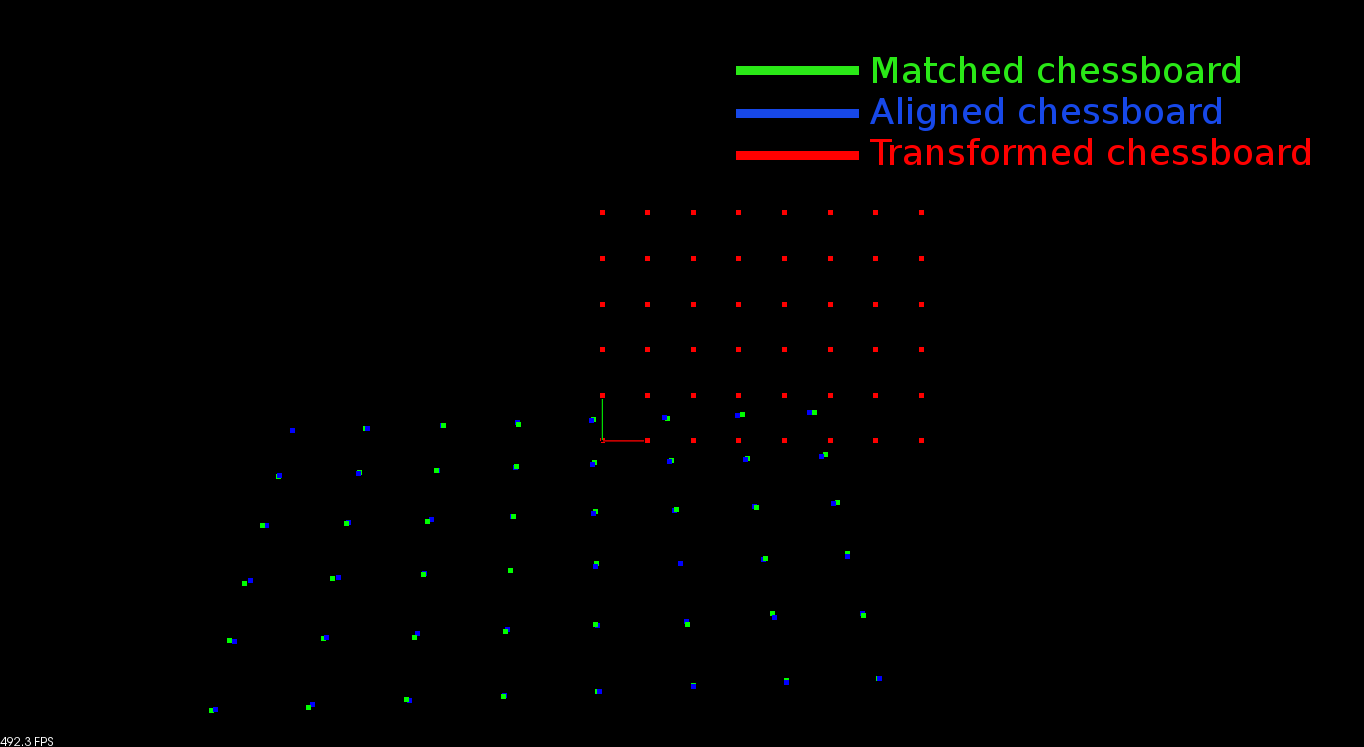
\includegraphics[width=2.5in]{./Results/Chessboard_alignment}}
\end{tabular}
\caption{Left: Chessboard's points are correctly found during calibration. Right: Chessboard's points are correctly aligned after full camera calibration.\label{fig:extr_alignment}}
\end{figure}
